%% Chapter 4

\cleardoublepage

\chapter{Development of Mathematical Models for NERMLAB}
\label{chp4}

Chapter \ref{chp4} will develop various mathematical models for the NERMLAB and Motorlab. These models are used throughout this thesis to help compare, analyis, and develop effective control solutions for motor controllers. Rather than have each experiment develop its own model in the corresponding chapter, it will be done here to help simplify the content of each experiment. Since the NERMLAB and Motorlab use different input sources \footnote{Nermlab uses voltage control. Motorlab uses current control.}, different mathematical models will be developed for each system seperately.

\section{Electrical Dynamics}
\label{electrical_dynamics}

\begin{figure}[H]
	\centering
	\caption[Electrical and Mechanical Schematic of NERMLAB]{Electrical and Mechanical Diagram of NERMLAB}
		% NERMLAB Circuit and Mechanical Diagram
	
	\tikzset{cross/.style={cross out, draw=black, minimum size=10*(#1-\pgflinewidth), inner sep=0pt, outer sep=0pt},
	%default radius will be 1pt. 
		cross/.default={0.9pt}}
	\centering
	\begin{circuitikz} \draw
		(0,0) to [V, v=$V$, *-*] (0,2) 
		to [R, l=$R$] (2,2)
		to [L, l=$L$,i^=$i$] (4,2)
		to [V, v_<=$K_e\omega$] (4,0) to [generic] (4,2) -- (4,0) -- (0,0);
	\end{circuitikz}
	\hspace{-0.3cm}
	\begin{tikzpicture}[scale=1]
		\draw [thick] (-1.5,.7) -- (-0.45,.7);
		\node[text width=3cm] at (1.7,0.75) {\Large $J$};
		\node[text width=3cm] at (1.1,-0.06) {$b$};
		\draw [thick] (-0.1,-0.16) -- (1.4,-0.16);
		\draw (0,-0.08) node[cross,rotate=2] {};
		\draw (0.1,-0.08) node[cross,rotate=2] {};
		\draw (0.2,-0.08) node[cross,rotate=2] {};
		\draw (0.3,-0.08) node[cross,rotate=2] {};
		\draw (0.4,-0.08) node[cross,rotate=2] {};
		\draw (0.5,-0.08) node[cross,rotate=2] {};
		\draw (0.6,-0.08) node[cross,rotate=2] {};
		\draw (0.7,-0.08) node[cross,rotate=2] {};
		\draw (0.8,-0.08) node[cross,rotate=2] {};
		\draw (0.9,-0.08) node[cross,rotate=2] {};
		\draw (1,-0.08) node[cross,rotate=2] {};
		\draw (1.1,-0.08) node[cross,rotate=2] {};
		\draw (1.2,-0.08) node[cross,rotate=2] {};
		\draw [thick] (0,1.5)  -- (0.2,1.5);
		\draw [thick] (0,0)  -- (0.2,0);
		\draw [thick](0,0) to [out=180, in=180] (0,1.5);
		\draw [thick] (0.2,0) to [out=180, in=180] (0.2,1.5);
		\draw [thick] (0.3,0) to [out=180, in=180] (0.3,1.5);
		\draw [thick] (0.3,0) -- (1.3,0);
		\draw [thick] (0.3,1.5) -- (1.3,1.5);
		\draw [thick] (1.3,0) to [out=0, in=0] (1.3,1.5);
		\draw [thick] (1.3,0) to [out=180, in=180] (1.3,1.5);
		\draw [thick] (1.35,.60) to [out=0, in=0] (1.35,.85);
		\draw [thick] (1.35,.60) to [out=180, in=180] (1.35,.85);
		\draw [->, dashed, thick] (0.6,-0.1) to [out=180, in=180] (0.6,1.6) node[above]{$\theta$}; 
		\draw [->, dashed, thick] (1.2,-0.1) to [out=180, in=180] (1.2,1.6) node[above right]{$T=k_Ti$}; 
	\end{tikzpicture}
	\label{nermlab_electrical_mechanical_diagram}
\end{figure}

The electrical dynamics play an important role in motor control when voltage is being used as an input to the system. Using Kirchoff's voltage law it is possible to find the dynamics of figure \ref{nermlab_electrical_mechanical_diagram}.

\[\sum V = 0\]


\[V(t) = Ri(t) + \cancelto{0}{L\frac{di}{dt}} + K_e\omega = Ri(t) + K_e\omega\]


\begin{equation}
\label{v_sum_equation}
V(t) = Ri(t) + K_e\omega
\end{equation}

Because the pole at -$\frac{R}{L}$ (6596.3 $\frac{rad}{s}$) is 10 times as large as the other dynamics of the system, it can be ignored in the analysis process. From equation \ref{v_sum_equation}, it is now possible to derive an equation for the output torque of the system in terms of supplied voltage.

\begin{equation}
\label{kt_equation}
T = k_Ti(t) \Leftrightarrow i(t) = \frac{T(t)}{k_T}
\end{equation}

Using equations \ref{kt_equation} and \ref{v_sum_equation}, equation \ref{torque_equation} and \ref{current_equation} can be derived, respectively.

\begin{equation}
\label{torque_equation}
T(t) = \frac{k_T}{R}(V(t)-K_e\omega)
\end{equation}

\begin{equation}
\label{current_equation}
i(t) = \frac{V(t)-K_e\omega}{R}
\end{equation}


\section{Combined Dynamics - Electrical and Mechanical}
\label{mechanical_dynamics}
Section \ref{mechanical_dynamics} will detail the model development for the various electro-mechanical models that are used throughout this thesis. Subsections \ref{position_models} and \ref{speed_models} will derive mathematical models for position and speed systems, respectively, with different input sources. For the model derivations using current as an input source, the closed-loop current control system is assumed to be much faster than the mechanical dynamics. As a result of this assumption only the mechanical dynamics and controller will be in the model development.


\subsection{Position Models}
\label{position_models}

\begin{figure}[H]
	\tikzset{cross/.style={cross out, draw=black, minimum size=10*(#1-\pgflinewidth), inner sep=0pt, outer sep=0pt},
		%default radius will be 1pt. 
		cross/.default={1.3pt}}
	\begin{center}
		\caption[Position Model]{Position Model}
		\label{model_chp4}
		\begin{tikzpicture}[scale=2]
\node[text width=3cm] at (1.1,0.75) {\Large $J$};
\node[text width=3cm] at (0.5,-0.06) {$b$};
\draw [thick] (-0.1,-0.16) -- (1.4,-0.16);
\draw (0,-0.08) node[cross,rotate=2] {};
\draw (0.1,-0.08) node[cross,rotate=2] {};
\draw (0.2,-0.08) node[cross,rotate=2] {};
\draw (0.3,-0.08) node[cross,rotate=2] {};
\draw (0.4,-0.08) node[cross,rotate=2] {};
\draw (0.5,-0.08) node[cross,rotate=2] {};
\draw (0.6,-0.08) node[cross,rotate=2] {};
\draw (0.7,-0.08) node[cross,rotate=2] {};
\draw (0.8,-0.08) node[cross,rotate=2] {};
\draw (0.9,-0.08) node[cross,rotate=2] {};
\draw (1,-0.08) node[cross,rotate=2] {};
\draw (1.1,-0.08) node[cross,rotate=2] {};
\draw (1.2,-0.08) node[cross,rotate=2] {};
\draw [thick] (0,1.5)  -- (0.2,1.5);
\draw [thick] (0,0)  -- (0.2,0);
\draw [thick](0,0) to [out=180, in=180] (0,1.5);
\draw [thick] (0.2,0) to [out=180, in=180] (0.2,1.5);
\draw [thick] (0.3,0) to [out=180, in=180] (0.3,1.5);
\draw [thick] (0.3,0) -- (1.3,0);
\draw [thick] (0.3,1.5) -- (1.3,1.5);
\draw [thick] (1.3,0) to [out=0, in=0] (1.3,1.5);
\draw [thick] (1.3,0) to [out=180, in=180] (1.3,1.5);
\draw [thick] (1.35,.60) to [out=0, in=0] (1.35,.85);
\draw [thick] (1.35,.60) to [out=180, in=180] (1.35,.85);
\draw [->, dashed, thick] (0.6,-0.1) to [out=180, in=180] (0.6,1.6) node[above]{$\theta$}; 
\draw [->, dashed, thick] (1.2,-0.1) to [out=180, in=180] (1.2,1.6) node[above]{$T$}; 
\end{tikzpicture}
	\end{center}
\end{figure}

The best way to start the formulation is to begin with a time domain differential equation of the mechanical system. Because the system is composed of only an angular mass and viscous friction (figure \ref{model_chp4}), a describing differential equation can be written as such.

\begin{equation} \label{dynamic_equation_1}
T = k_T i(t) = b \dot \theta(t) + J \ddot \theta(t)
\end{equation}

Taking the Laplace transform of equation \ref{dynamic_equation_1}:
\begin{equation} \label{laplace_transform_1}
k_T I(s) = (bs + Js^2)\theta(s)
\end{equation}

The transfer function can then be developed for $G_m$ from equation \ref{laplace_transform_1}.
\begin{equation}
\label{motorlab_position_equation}
\frac{\theta(s)}{I(s)} = \frac{k_T}{Js^2 + bs}
\end{equation}


\subsubsection{Position Model - Voltage as Input}
Equation \ref{motorlab_position_equation} adequately describes the system for the Motorlab because the electrical dynamics are much faster than the mechanical. However in the case of the NERMLAB, voltage control is used and the same can not be said, and as a result, a different model must be developed. Starting with the differential equations of the electrical dynamics and mechanical dynamics, the following equations are found.

\begin{equation}
\label{starting_electrical_equation}
V(t) = Ri(t) + L\frac{di}{dt} + K_e \dot{\theta}(t)
\end{equation}

\begin{equation}
\label{starting_mechanical_equation}
T(t) = J\ddot{\theta}(t) + b \dot{\theta}(t)
\end{equation}

Taking the Laplace transform of equations \ref{starting_electrical_equation} and \ref{starting_mechanical_equation}.

\begin{equation}
\label{electrical_laplace}
V(s) = RI(s) + LsI(s) + K_e s \theta(s)
\end{equation}

\begin{equation}
\label{mechanical_laplace}
T(s) = (Js^2 + bs)\theta(s)
\end{equation}

From section \ref{electrical_dynamics}, the relationship between torque and current is known. Substituting equation \ref{kt_equation} into equation \ref{mechanical_laplace}, an equation for current is found.

\begin{equation}
\label{current equation}
I(s) = \frac{(Js^2 + bs)}{k_T}\theta(s)
\end{equation}

Subtituting equation \ref{current_equation} into equation \ref{electrical_laplace}, grouping and finding a common denominator in the process, yields equation \ref{final_equation_with_L}.

\begin{equation}
\label{final_equation_with_L}
\frac{\theta(s)}{V(s)} = \frac{k_T}{(Ls+R)(Js^2 + bs) + K_ek_Ts}
\end{equation}

As stated in section \ref{electrical_dynamics}, the electrical dynamics involving $L$ are much larger than any other dynamics in the system, therefore L can be ignored, resulting in the final position equation in terms of voltage as an input source.

\begin{equation}
\label{position_equation_voltage}
\frac{\theta(s)}{V(s)} = \frac{k_T}{RJs^2 + (Rb + K_ek_T)s}
\end{equation}

\subsection{Speed Models}
\label{speed_models}

\begin{figure}[H]
	\tikzset{cross/.style={cross out, draw=black, minimum size=10*(#1-\pgflinewidth), inner sep=0pt, outer sep=0pt},
		%default radius will be 1pt. 
		cross/.default={1.3pt}}
	\begin{center}
		\caption[NERMLAB Speed Model]{NERMLAB Speed Model}
		\label{model_speed_chp4}
		\begin{tikzpicture}[scale=2]
\node[text width=3cm] at (1.1,0.75) {\Large $J$};
\node[text width=3cm] at (0.5,-0.06) {$b$};
\draw [thick] (-0.1,-0.16) -- (1.4,-0.16);
\draw (0,-0.08) node[cross,rotate=2] {};
\draw (0.1,-0.08) node[cross,rotate=2] {};
\draw (0.2,-0.08) node[cross,rotate=2] {};
\draw (0.3,-0.08) node[cross,rotate=2] {};
\draw (0.4,-0.08) node[cross,rotate=2] {};
\draw (0.5,-0.08) node[cross,rotate=2] {};
\draw (0.6,-0.08) node[cross,rotate=2] {};
\draw (0.7,-0.08) node[cross,rotate=2] {};
\draw (0.8,-0.08) node[cross,rotate=2] {};
\draw (0.9,-0.08) node[cross,rotate=2] {};
\draw (1,-0.08) node[cross,rotate=2] {};
\draw (1.1,-0.08) node[cross,rotate=2] {};
\draw (1.2,-0.08) node[cross,rotate=2] {};
\draw [thick] (0,1.5)  -- (0.2,1.5);
\draw [thick] (0,0)  -- (0.2,0);
\draw [thick](0,0) to [out=180, in=180] (0,1.5);
\draw [thick] (0.2,0) to [out=180, in=180] (0.2,1.5);
\draw [thick] (0.3,0) to [out=180, in=180] (0.3,1.5);
\draw [thick] (0.3,0) -- (1.3,0);
\draw [thick] (0.3,1.5) -- (1.3,1.5);
\draw [thick] (1.3,0) to [out=0, in=0] (1.3,1.5);
\draw [thick] (1.3,0) to [out=180, in=180] (1.3,1.5);
\draw [thick] (1.35,.60) to [out=0, in=0] (1.35,.85);
\draw [thick] (1.35,.60) to [out=180, in=180] (1.35,.85);
\draw [->, dashed, thick] (0.6,-0.1) to [out=180, in=180] (0.6,1.6) node[above]{$\omega$}; 
\draw [->, dashed, thick] (1.2,-0.1) to [out=180, in=180] (1.2,1.6) node[above]{$T$}; 
\end{tikzpicture}
	\end{center}
\end{figure}

The position models just developed in section \ref{position_models} can be used to help derive models for speed. The process is a relatively straight forward one, with one simple substitution needed. Knowing the relationship between speed and position, it is possible to write the following equation.

\begin{equation}
\label{theta_speed_rel}
\theta(s) = \frac{\omega(s)}{s}
\end{equation}

Substituting equation \ref{theta_speed_rel} into \ref{motorlab_position_equation} simply cancels the free integrator, leaving the final equation in terms of speed.

\begin{equation}
\label{motorlab_speed_equation}
\frac{\omega(s)}{I(s)} = \frac{k_T}{Js + b}
\end{equation}

\subsubsection{Speed Model - Voltage as Input}

Just as in section \ref{speed_models}, a simple substitution of equation \ref{theta_speed_rel} into \ref{position_equation_voltage} yields the final speed model in terms of voltage.

\begin{equation}
\label{speed_equation_voltage}
\frac{\omega(s)}{V(s)} = \frac{k_T}{RJs + (Rb + K_ek_T)}
\end{equation}


\subsection{Pendulum Model}

The pendulum model is a mathematical formulation for NERMLAB that is used to help find the resonant frequency. It should be noted that the dynamic equations for this setup are non-linear in nature, and as a result, the small angle approximation ($sin(\theta) \approx \theta$) must be used in order to transform the time dependent system into the frequency domain. The small angle approximation is only valid for angles that are smaller than 0.244 radians, as the relative error between $sin(\theta)$ and $\theta$ exceeds 1 percent at this value. This will be taken into account when running experiments on the NERMLAB system.

\begin{figure}[H]
	\tikzset{cross/.style={cross out, draw=black, minimum size=10*(#1-\pgflinewidth), inner sep=0pt, outer sep=0pt},
		%default radius will be 1pt. 
		cross/.default={1.3pt}}
	\begin{center}
		\caption[NERMLAB Pendulum Model]{NERMLAB Pendulum Model}
		\label{model_pendulum_chp4}
			% NERMLAB Circuit and Mechanical Diagram
	
	\usetikzlibrary{calc,patterns,angles,quotes}
	
	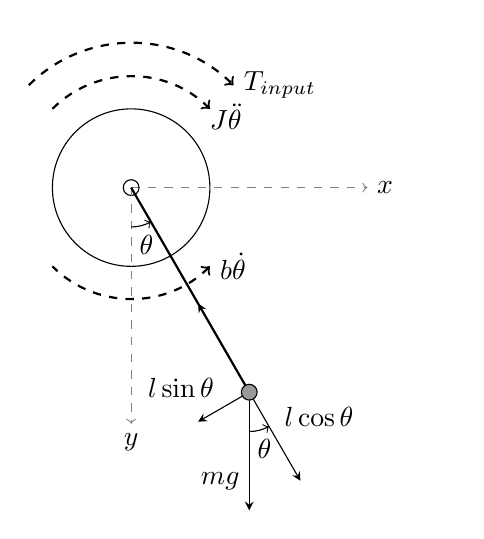
\begin{tikzpicture}[scale=1]	
 % save length of g-vector and theta to macros
 
 
 
\pgfmathsetmacro{\Gvec}{1.5}
\pgfmathsetmacro{\myAngle}{30}
% calculate lengths of vector components
\pgfmathsetmacro{\Gcos}{\Gvec*cos(\myAngle)}
\pgfmathsetmacro{\Gsin}{\Gvec*sin(\myAngle)}

\draw[->,dashed,gray] (0,0) -- ++ (3,0) node (mary) [black,right]{$x$};
\draw (0,0) circle (1cm);
\draw (0,0) circle (0.1cm);

\coordinate (centro) at (0,0);
\draw[->,dashed,gray] (centro) -- ++ (0,-3) node (mary) [black,below]{$y$};
\draw[thick] (centro) -- ++(270+\myAngle:3) coordinate (bob);
\pic [draw, ->, "$\theta$", angle eccentricity=1.5] {angle = mary--centro--bob};
\draw [black,-stealth] (bob) -- ($(bob)!\Gcos cm!(centro)$);
\draw [-stealth] (bob) -- ($(bob)!-\Gcos cm!(centro)$)
coordinate (gcos)
node[midway,above right] {$l\cos\theta$};
\draw [-stealth] (bob) -- ($(bob)!\Gsin cm!90:(centro)$)
coordinate (gsin)
node[midway,above left] {$l\sin\theta$};
\draw [-stealth] (bob) -- ++(0,-\Gvec)
coordinate (g)
node[near end,left] {$mg$};
\pic [draw, ->, "$\theta$", angle eccentricity=1.5] {angle = g--bob--gcos};
\filldraw [fill=black!40,draw=black] (bob) circle[radius=0.1];

\node[text width=3cm] at (2.5,0.9) {$J \ddot{\theta}$};
\draw [->, dashed, thick] (-1,1) to [out=45, in=135] (1,1); 
\draw [<-, dashed, thick] (1,-1) node[below,right]{$b \dot{\theta}$} to [out=-135, in=-45] (-1,-1) ; 
\draw [->, dashed, thick] (-1.3,1.3) to [out=45, in=135] (1.3,1.3) node[above,right]{$T_{input}$}; 
	\end{tikzpicture}
	\end{center}
\end{figure}

The best way to start the derivation is to find the describing differential equations for both the mechanical and electrical system. In the case of the pendulum setup, the electrical dynamics are simply the torque the motor provides the pendulum with, which was found in section \ref{electrical_dynamics}, equation \ref{torque_equation}.

\begin{equation}
\label{pendulum_starting_dynamics}
J \ddot{\theta}(t) = -mgl\theta(t) - b\dot{\theta}(t) + T_{input}
\end{equation}

Substituting the electrical motor torque (eq. \ref{torque_equation}), into equation \ref{pendulum_starting_dynamics}.

\begin{equation}
J \ddot{\theta}(t) = -mgl\theta(t) - b\dot{\theta}(t) + \frac{k_T}{R}(V(t)-K_e \dot{\theta}(t))
\end{equation}

\[J \ddot{\theta}(t) + mgl\theta(t) + b\dot{\theta}(t) + \frac{k_T K_e}{R}\dot{\theta}(t)= \frac{k_T}{R}V(t)\]

Taking the Laplace transform of the above equation yields:

\[(Js^2 + mgl + bs + \frac{k_T K_e}{R}s)\theta(s) = \frac{k_T}{R}V(s)  \]

\[\frac{JRs^2 + mglR + bRs + k_T K_es}{R}\theta(s) = \frac{k_T}{R}V(s) \]

\begin{equation}
\label{pendulum_model_unsimplified}
\frac{\theta(s)}{V(s)} = \frac{k_T}{JRs^2 + (bR + k_T K_e)s + mglR}
\end{equation}

Putting equation \ref{pendulum_model_unsimplified} into a standard second order form yields:

\begin{equation}
\label{pendulum_non_lumped}
\frac{\theta(s)}{V(s)} = \frac{\frac{k_T}{JR}}{s^2 + (\frac{b}{J} + \frac{k_T K_e}{JR})s + \frac{mgl}{J}}
\end{equation}

To further simplify the model, lumped coefficients for friction and the trailing term of equation \ref{pendulum_non_lumped} will be made since they are comprised of statically defined variables.

\begin{equation}
\label{lumped_friction}
b_l = \frac{b}{J} + \frac{k_T K_e}{JR}
\end{equation}

\begin{equation}
\label{lumped_wp}
\omega_p = \frac{mgl}{J}
\end{equation}

\begin{equation}
\label{lumped_kt}
k_{T,l} = \frac{k_T}{JR}
\end{equation}

\begin{equation}
\label{pendulum_model}
\frac{\theta(s)}{V(s)} = \frac{k_{T,l}}{s^2 + b_ls + \omega_p}
\end{equation}

It should be noted that $J$ is the pendulum's inertia and not the rotors in equation \ref{pendulum_model}; likewise, $l$ is the distance to the center of mass of the pendulum.
